\chapter{Mass-spectroscopy in protein structure determination}

This section introduces the two experimental methods, hydrogen exchange mass spectroscopy (HXMS) and cross-correlation mass spectroscopy (XCMS), and possible application in protein folding.

These experimental methods are attractive, since the experiments are relatively easy to carry out.

mass spectroscopy 

\section{Cross-linking mass spectroscopy (XLMS)}


XLMS has previously been used to 

We considered several linkers of different lengths. The \textit{de facto} standard linkers, DSS and DST which measure 11 \aa ngstr\"o m and 6.4 \aa ngstr\"o m, respectively.

\section{Hydrogen exchange mass spectroscopy (HXMS)}

\begin{figure}
    \centering
    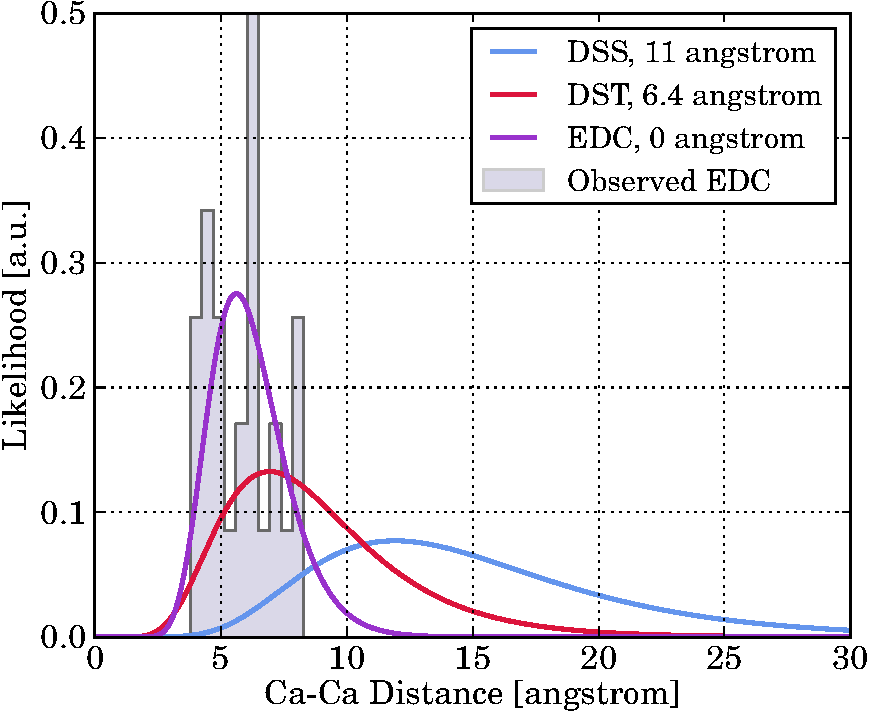
\includegraphics[width=0.65\textwidth]{figures/xcms/lognormal.pdf}
    \caption{linkers}
    \label{fig:linkers}
\end{figure}






